  %%%%%%%%%%%%%%%%%%%%%%%%%%%%%%%%%%%%%%% -*- coding: utf-8; mode: latex -*- %%
  %
%%%%%                       CHAPTER
 %%%
  %

% $Id: 3100-nihil-molestiae.tex,v 1.1 2007/11/23 09:52:43 david Exp $
% $Log: 3100-nihil-molestiae.tex,v $
% Revision 1.1  2007/11/23 09:52:43  david
% *** empty log message ***
%
%

  %%%%%%%%%%%%%%%%%%%%%%%%%%%%%%%%%%%%%%%%%%%%%%%%%%%%%%%%%%%%%%%%%%%%%%%%%%%%%
  %
%%%%%                    HEAD MATTER
 %%%
  %

\chapter{Evaluation}
%\addcontentsline{lof}{chapter}{\thechapter\quad Nihil Molestiae}
%\addcontentsline{lot}{chapter}{\thechapter\quad Nihil Molestiae}
\label{ch:evaluation}

%\begin{quotation}
%  {\small\it }
%
%{\small\it -- }
%\end{quotation}



  %%%%%%%%%%%%%%%%%%%%%%%%%%%%%%%%%%%%%%%%%%%%%%%%%%%%%%%%%%%%%%%%%%%%%%%%%%%%%
  %
%%%%%                        FIRST SECTION
 %%%
  %

\section{Testbed}
During evaluation of the QoD prototype a test-bed with several HBase cluster has been deployed at INESC-ID and IST in Lisbon, some of them with an HBaseQoD-enabled engine for quality of data between replicas, and others running a regular implementation of HBase 0.94.8. All tests were conducted using 6 machines with an Intel Core i7-2600K CPU at 3.40GHz, 11926MB of available RAM memory, and HDD 7200RPM SATA 6Gb/s 32MB cache, connected by 1 Gigabit LAN and we expect to continue obtaining results using a network tool as~\cite{netem:2005} for delaying and simulating network bandwidth and latency between a distant set of locations. We are also currently trying to confirm that the appropriate QoD does have a positive impact when bounding staleness (monitoring time an pending updates, instead of number of updates) with varying delays, but not now due to space constraints in this text, we do not present it. Even though, it is obvious this will just spread replication activity in time, but expecting a reduced max-value on each network peak-load observed.


\section{Experiments}

\begin{figure}[h]
\centering
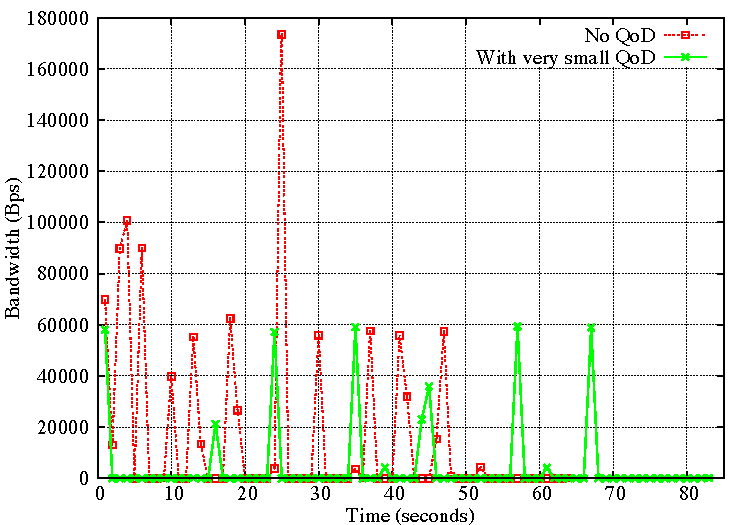
\includegraphics[width=0.8\textwidth]{figs/bandwidth.pdf}
\caption{Bandwidth usage and replication frequency for a typical workload with and very small HBase-QoD constraint for K($\sigma$)}
\label{fig-bw-freq}
\end{figure}

In Figure~\ref{fig-bw-freq} for a very small QoD of K using $\sigma$ we realize that there is a lower limit where latency can not be reduced any further. We have measured that same value in the subsequent Figure~\ref{fig-bandwidth-worloada-modified} with a larger QoD of K using $\sigma$ = 0.5\%. Recall this means the percentage of records allowed to be modified, or of updates applied in relation to total number of records, before replication is triggered (a very small value, where strict consistency would mean 0.00\%).

We can see the bandwidth peaks and therefore measure average usage of the former, which decreases with the increase of the QoD bound in the order of magnitude of 1MB per second as we experimentally verify from the graphs obtained. That is due to the batching of updates in our vector model, so items are not replicated until one of the constraints time, sequence or value is met. Basically, overall we can see less communication between clusters at replication time increasing QoD, which is a good measurement of how one can optimize bandwidth. During that time then we take advantage of our caching mechanisms inside QoD while sending all the information demanded in a timely fashion once data becomes necessary to the application.

%In Figure 1, we appreciated that our QoD helps to control peak bounds of updates, and therefore the eventual consistency approach of leaving replication of the items at the odds of the RPC mechanisms of the system in question. We %can control that, and the graph shows how a maximum threshold of around 1000 is constantly reached for the modified version of HBase, but no more. Obviously the timespan of updates with QoD might be longer depending of the values %chosen, but that is a built-in property of our work on purpose for only propagating updates when they are strictly necessary and to satisfy a given SLO.

\begin{figure}[h]
\centering
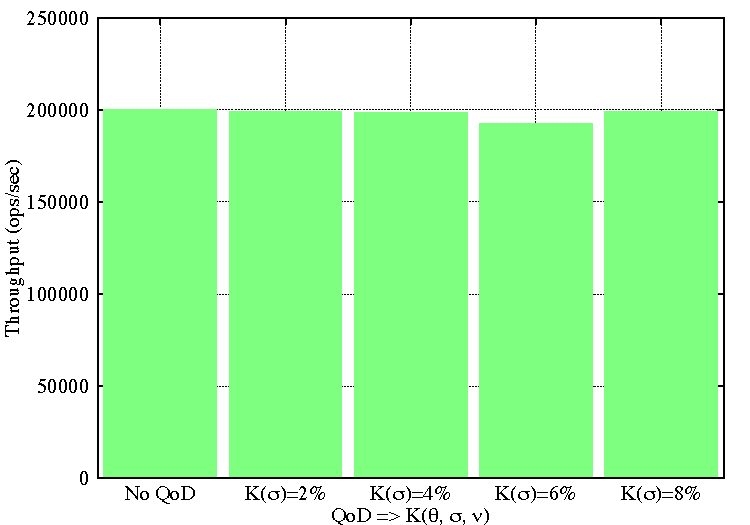
\includegraphics[width=0.8\linewidth]{figs/throughput.pdf}
\caption{Throughput for several QoD configurations}
\label{fig-throughput}
\end{figure}
We also confirm the QoD does not hurt performance as we observe from the throughput achieved for the several levels of QoD chosen during the evaluation of the throughput achieve with the benchmark for our modified version with HBase=QoD enabled, Figure~\ref{fig-throughput}. The differences in throughput are irrelevant and mostly due to noise in the network, that is the conclusion after obtaining similar results to that one in several rounds of tests with the same input workload on the data store.

Next we conducted as shown in Figure~\ref{fig-cpu}, and \emph{dstat} presents, an experiment to monitor the CPU usage using HBase-QoD. CPU consumption and performance remains roughly the same and therefore stable in the cluster machines as can be appreciated.
\begin{figure}[h]
\centering
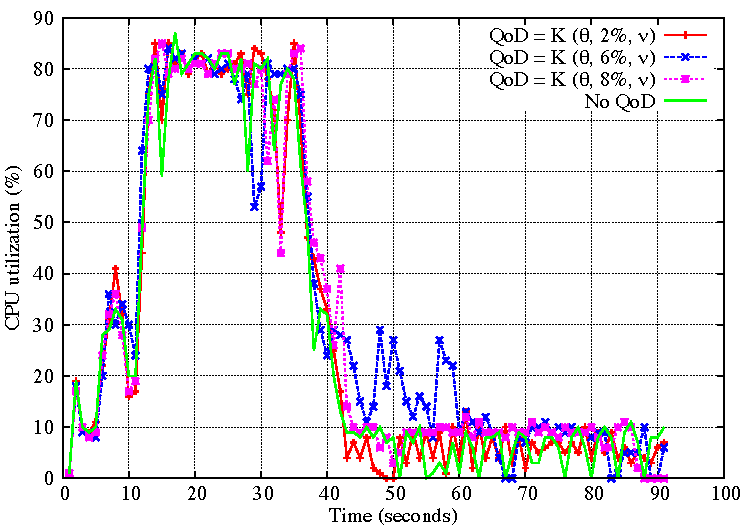
\includegraphics[width=0.8\linewidth]{figs/cpu.pdf}
\caption{CPU usage over time with QoD enabled}
\label{fig-cpu}
\end{figure}

%In Figure 4 (for batches of updates of 5M) we can see the bandwidth peaks and therefore measure average usage of the former, which decreases with the increase of the QoD bound in the order of magnitude of 1MB per second as we %experimentally verify from the graphs obtained. That is due to the batching of updates in our vector model, so items are not replicated until one of the constraints time, sequence or value is met. Basically, overall we can see %less communication between clusters at replication time increasing QoD, which is a good measurement of how one can optimize bandwidth while non-key data semantics are presented to the application at a required instant in time but %not earlier if not critical. During that time then we take advantage of our caching mechanisms inside QoD while sending all the information demanded in a timely fashion once data becomes necessary to the application.

We have also taken measurements for the following workloads obtaining results as follows:

\subsection{Workloads for YCSB}

We have tested our implementation in HBase with several built-in workloads from YCSB plus one customer workload with 100\% writes to stress the database intensively as the target updates in the social network previously described is about changes and new insertions.

Figure~\ref{fig-bandwidth-worloada} shows three different sets of Qualities of Data for the same workload (A):

\begin{enumerate}
\item{YCSB workload A (R/W - 50/50)}
	\begin{itemize}
		\item No QoD enforced.
		\item QoD fulfillment of $\sigma$=0.5\% of total updates to be replicated.
		\item QoD fulfillment of $\sigma$=2\% of total updates to be replicated.
	\end{itemize}

During the execution of the workload A, in Figure~\ref{fig-bandwidth-worloada}, the highest peaks in replication traffic are observed without any type of QoD, i.e. just using plain HBase. This is due to the nature of eventual consistency itself and the buffering mechanisms in HBase.

With a QoD enabled as shown in the other two graphs, we rather control traffic of updates from being unbounded to a limited amount, accordingly to save resources' utilization, while suiting applications that require small amounts of information to be only propagated as a group, when they are just needed.

We observe that higher QoD requires replication traffic less frequently, although interactions reach higher values on Bytes as they need to send more data. Small QoD optimizes the usage of resources while sending priority updates more frequently (this could be the case of wall posts in a social network).

\begin{figure*}
\centering
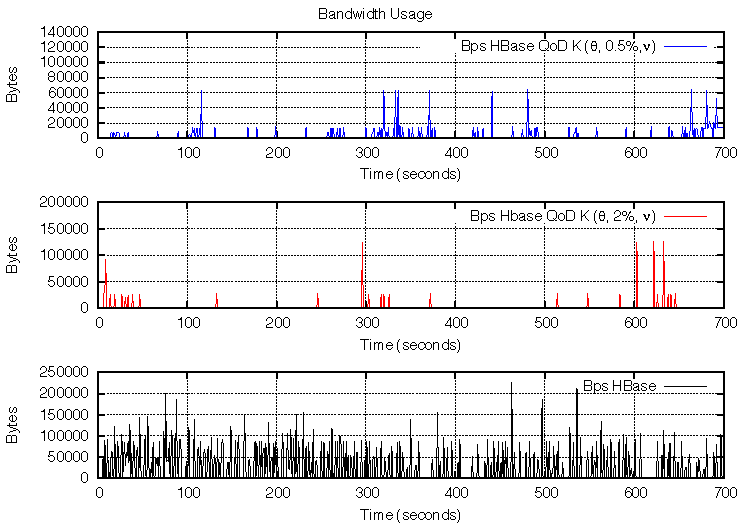
\includegraphics[width=0.8\linewidth]{figs/plot-packets-size-workloada-allbounds-latest.pdf}
\caption{Bandwidth usage for Workload A using 5M records using QoD bounds of 0.5 and 2\% in the $\sigma$ of K.}
\label{fig-bandwidth-worloada}
\end{figure*}

\item{YCSB workload A modified (R/W - 0/100)}
	\begin{itemize}
		\item No QoD enforced.
		\item QoD fulfillment of $\sigma$=0.5\% of total updates to be replicated.	% 25K updates (5M total)
		\item QoD QoD fulfillment of $\sigma$=2\% of total updates to be replicated.  % 100K updates (5M total)
	\end{itemize}
\end{enumerate}

\begin{figure*}
\centering
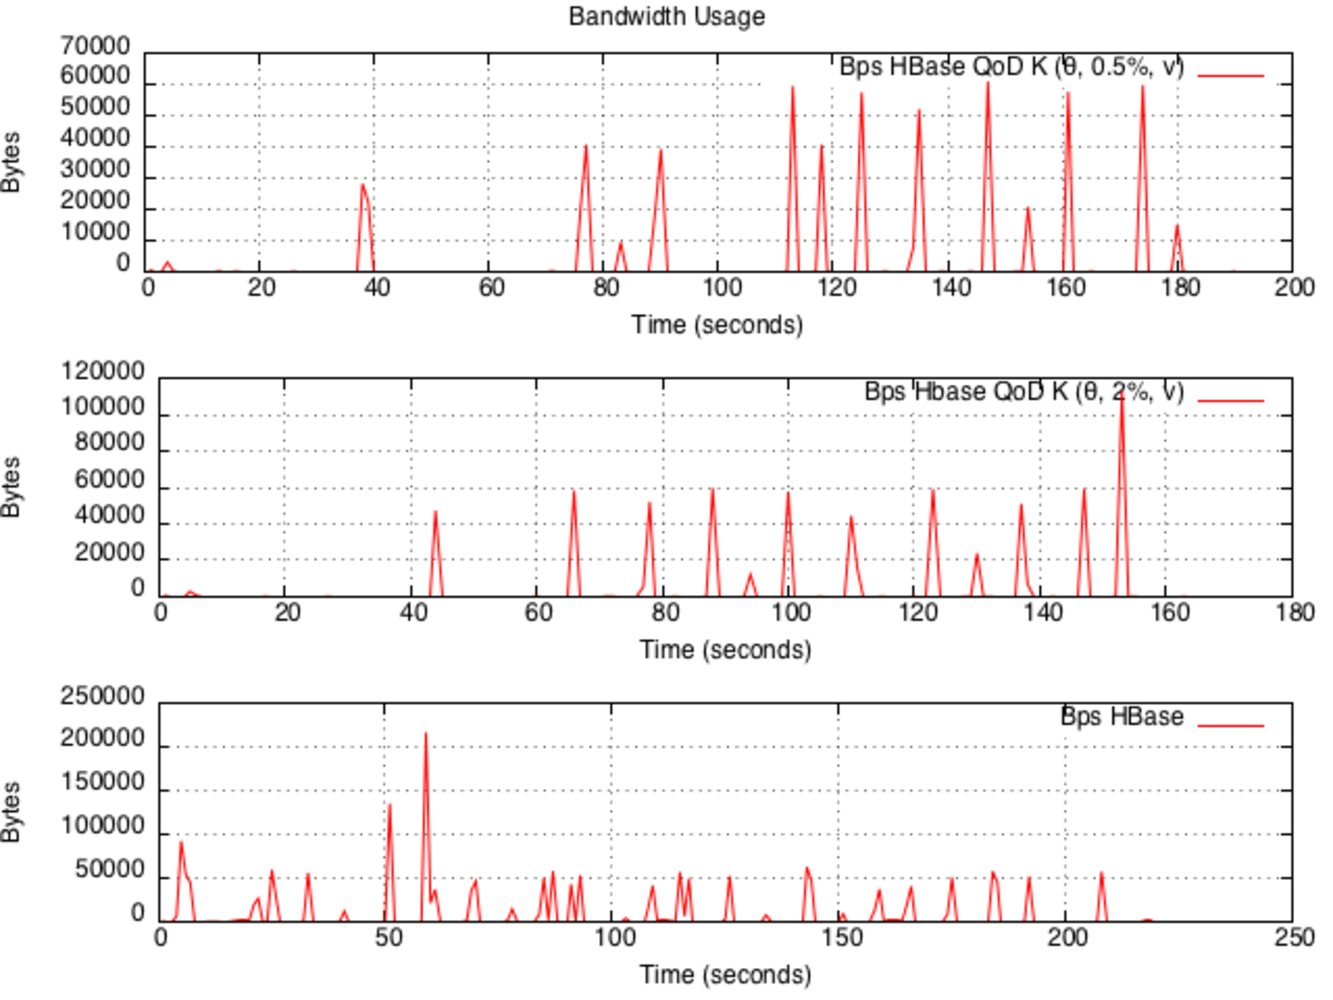
\includegraphics[width=0.8\linewidth]{figs/plot-packets-size-workloada-modified-allbounds-30threads.pdf}
\caption{Bandwidth usage for Workload A-Modified using 5M records using QoD bounds of 0.5 and 2\% in the $\sigma$ of K.}
\label{fig-bandwidth-worloada-modified}
\end{figure*}

In Figure ~\ref{fig-bandwidth-worloada-modified} we can see how a write intensive workload performs using a QoD. Similar results are expected and later also confirmed in this graph (please note the scale of the Y axis is modified in order to show the relevant difference in Bytes more accurately).
  For smaller QoD (0.5\%) we see lower peaks in bandwidth usage, as well as in the following measurement used (2.0\%). Finally HBase with no modifications shows a much larger number of Bytes when coming to maximum bandwidth consumption.
 
 Note we are not measuring, or find relevant, in any of these scenarios, to realize any kind of claims based on average bandwidth usage. The principal source of motivation of the paper is to find a way of controlling the usage of the resources in a data center, by ensuring a uniform distribution of replication of updates across time. Also, to be able to trade strong consistency for groups of operations treated atomically, for shipment to the destination cluster location at a given point in time, or when the data-semantics bound is reached. 


